\documentclass[titlepage,article,paper=b4,twocolumn]{jlreq}
\setlength{\columnseprule}{0.5pt}
\setlength{\columnsep}{5\zw}
\usepackage[top=30mm,bottom=20mm,left=15mm,right=15mm]{geometry}
\usepackage{amssymb,mathtools,mathcomp}
\usepackage{enumitem,tasks}
\usepackage{physics,physics2}
\settasks{label-width=2\zw}
\usephysicsmodule{ab,ab.braket}
\usepackage{bm}
\usepackage{graphicx,tabularx,here}
\usepackage{tikz,tikz-3dplot}
\usetikzlibrary{math,angles,quotes,calc,intersections}
\usepackage{kyotsutest}
\usepackage{answerbox}
\usepackage[pdftitle={中３数学１学期期末解答},pdfauthor={まさし},hidelinks]{hyperref}
\newcommand{\Div}{\mathbin{\textrm{\textdiv}}}

\NewPageStyle{examMA}
{nombre_position=top-left,
nombre={\Large{$\smash{\raisebox{-0.5\zh}{\href{https://fanme.link/@masashi\_00\_}{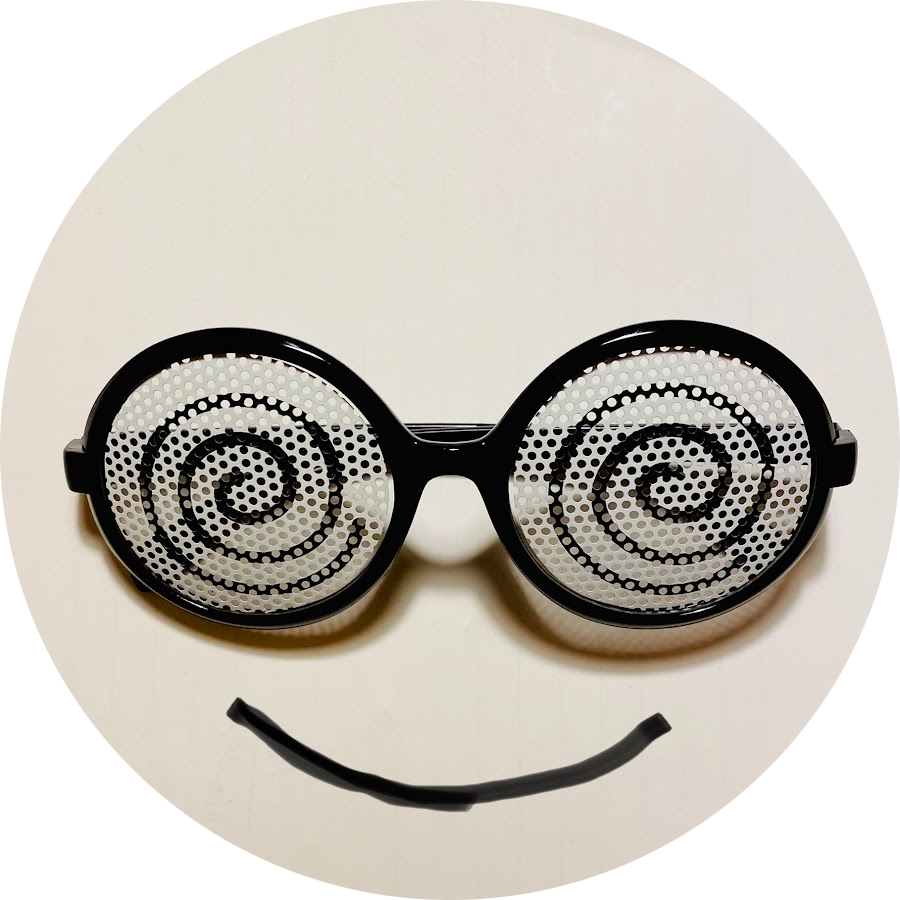
\includegraphics[width=2.5\zw]{../../common/icon-masashi.png}}}}$ 中学３年 数学 １学期期末対策 模範解答\quad\textrm{No.~\thepage}}},
running_head_position=top-right,
odd_running_head=\normalsize{\textrm{３年\underline{\hspace{2\zw}}組\underline{\hspace{2\zw}}番
\hspace{0.5\zw}氏名\underline{\hspace{15\zw}}}}}

\begin{document}
\pagestyle{examMA}
\setcounter{page}{1}

\begin{ansbox}
\pbox[3]{5}
\ptxt{1}{l}{\quad $\pm 2$}
\ptxt{2}{l}{\quad $\pm\sqrt{11}$}
\ptxt{3}{l}{\quad $\pm 0.4$}
\ptxt{4}{l}{\quad $\pm\dfrac{5}{7}$}
\ptxt{5}{l}{\quad $\pm \sqrt{5}$}
\end{ansbox}

\begin{ansbox}
\pbox{3}
\ptxt{1}{l}{\quad $6$}
\ptxt{2}{l}{\quad $-7$}
\ptxt{3}{l}{\quad $11$}
\end{ansbox}

\begin{ansbox}
\pbox[2]{7}
\ptxt{1}{l}{\quad $2\sqrt{3}$}
\ptxt{2}{l}{\quad $18\sqrt{10}$}
\ptxt{3}{l}{\quad $\sqrt{3}$}
\ptxt{4}{l}{\quad $\sqrt{3}$}
\ptxt{5}{l}{\quad $0$}
\ptxt{6}{l}{\quad $4\sqrt{2}$}
\ptxt{7}{l}{\quad $7\sqrt{2} - 2\sqrt{3}$}
\end{ansbox}

\begin{ansbox}
\pbox[2]{7}
\ptxt{1}{l}{\quad $x = \pm\sqrt{6}$}
\ptxt{2}{l}{\quad $x = 0,\,-11$}
\ptxt{3}{l}{\quad $x = 7,\,-8$}
\ptxt{4}{l}{\quad $x = -3$}
\ptxt{5}{l}{\quad $x = \dfrac{2\pm\sqrt{13}}{9}$}
\ptxt{6}{l}{\quad $x = -1,\,-\dfrac{7}{6}$}
\ptxt{7}{l}{\quad $x = -\dfrac{10}{3},\,\dfrac{11}{3}$}
\end{ansbox}

\begin{ansbox}
\pbox{5}
\ptxt{1}{c}{\batsu}
\ptxt{2}{c}{\maru}
\ptxt{3}{c}{\maru}
\ptxt{4}{c}{\batsu}
\ptxt{5}{c}{\batsu}
\end{ansbox}

\begin{ansbox}
\pbox{2}
\ptxt{1}{l}{\quad $25$}
\ptxt{2}{l}{\quad $31$}
\pbox{1}
\ptxt{3}{l}{\quad $2,\,3,\,5,\,7,\,11,\,13,\,17,\,19$}
\end{ansbox}

\begin{ansbox}
\pbox[1]{3}
\ptxt{1}{l}{\quad $n = 5,\,6$}
\ptxt{2}{l}{\quad $n = 2,\,7,\,10,\,11$}
\ptxt{3}{l}{\quad $n = 2$}
\end{ansbox}

\begin{ansbox}
\pbox*{2}
\ptxt{1}{l}{\quad $a = -9$}
\ptxt{2}{l}{\quad 他の解：\ $x = 7$}
\end{ansbox}

\begin{ansbox}
\pbox*[3]{1}
\ptxt{1}{l}{\quad $4$}
\end{ansbox}

\begin{ansbox}
\pbox*[3]{1}
\ptxt{1}{r}{\quad\hfill$1$\hfill$\textrm{m}$\hspace{\zw}}
\end{ansbox}
\newpage

\begin{ansbox}[height=120mm]
\pbox*{1}
\ptxt{1}{c}{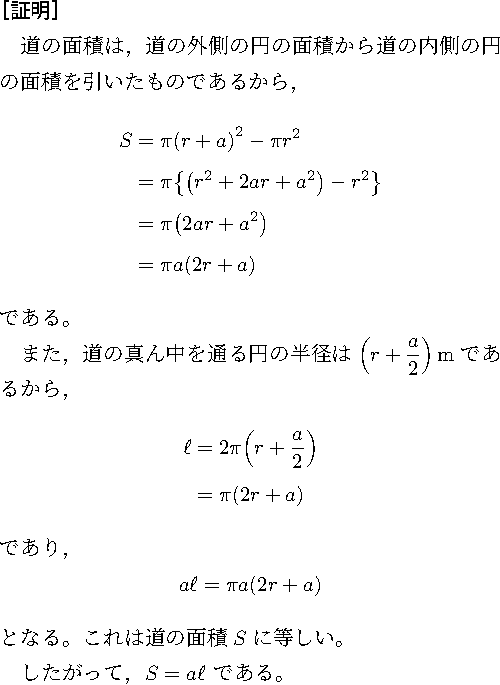
\includegraphics[width=0.8\linewidth]{fig/証明/3-1-f-1.pdf}}
\end{ansbox}

\begin{ansbox}[height=90mm]
\pbox*{1}
\ptxt{1}{c}{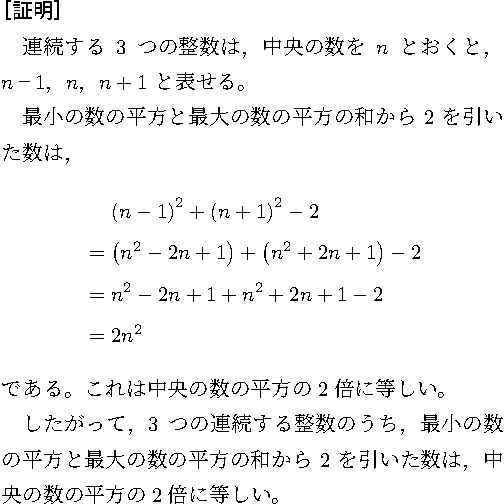
\includegraphics[width=0.8\linewidth]{fig/証明/3-1-f-2.pdf}}
\end{ansbox}

\vfill
\hfill{}まさしの情報はここからチェック → \href{https://fanme.link/@masashi\_00\_}{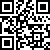
\includegraphics[width=3\zw]{../../common/qr-fanme.png}}
\newpage

\noindent\textbf{［補足］}\newline
5. (5) $\sqrt{-64}$ は高校で扱う。虚数単位$\mathrm{i}$を用いて $8\mathrm{i}$ と表される。\newline
7. (2) $\sqrt{0} = 0$ で整数となるため，$n = 11$ も含まれる。\newline
9. もとの数は自然数であることに注意する。\newline
12. 連続する3つの整数を $n$，$n + 1$，$n + 2$ としてもよい。

\newpage

\noindent\textbf{［配点］}\newline
\textbf{1.} 10点（各2点）\newline
\textbf{2.} 6点（各2点）\newline
\textbf{3.} 21点（各3点）\newline
\textbf{4.} 21点（各3点）\newline
\textbf{5.} 5点（各1点）\newline
\textbf{6.} 8点（(1), (2) 各3点，(3) 2点）\newline
\textbf{7.} 6点（(1), (2), (3) 各2点）\newline
\textbf{8.} 4点（各2点）\newline
\textbf{9.} 3点\newline
\textbf{10.} 4点\newline
\textbf{11.} 6点\newline
\textbf{12.} 6点\newline

\vfill
\hfill{}まさしの情報はここからチェック → \href{https://fanme.link/@masashi\_00\_}{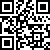
\includegraphics[width=3\zw]{../../common/qr-fanme.png}}
\end{document}